\section{Evaluation Metrics} \label{eval}

Text-to-SQL tasks can be evaluated by multiple methods: Component Matching, Accurate matching rate and Execution accuracy rate. Predicted SQL statements are compared with standard statements to determine how accurate the match is.
By splitting the predicted SQL statement and definitive statement into multiple clauses according to keywords, we can solve the problem of matching errors caused by the order of the where clause. The matching is successful as long as the elements in both sets are the same.

% pics/acc1.png
\begin{figure}[htb]
    \centering
    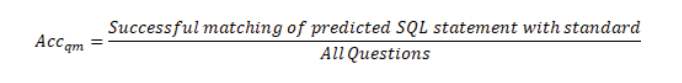
\includegraphics[width=0.6\textwidth]{pics/acc1.png}
    % \caption{Accurate matching rate}
    \label{fig:acc1}
\end{figure}

When using the correct predicted SQL statements, the correct execution rate refers to the proportion of questions that can receive the correct answers from the database.

% pics/acc2.png
\begin{figure}[htb]
    \centering
    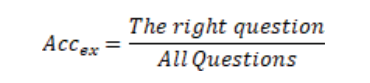
\includegraphics[width=0.4\textwidth]{pics/acc2.png}
    % \caption{Accuracy rate of the predicted SQL statements}
    \label{fig:acc2}
\end{figure}

% By predicting the key F1 values for SQL statements, the model can also be evaluated.

% % pics/f1.png
% \begin{figure}[htb]
%     \centering
%     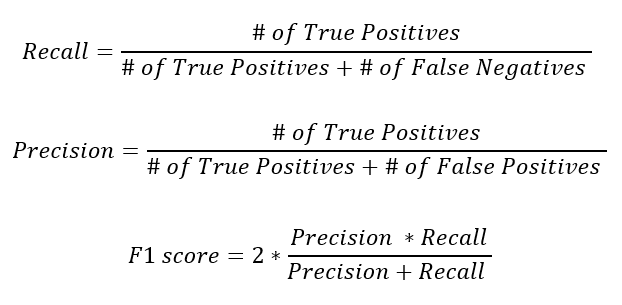
\includegraphics[width=0.6\textwidth]{pics/f1.png}
%     % \caption{F1 score for SQL statements}
%     \label{fig:f1}
% \end{figure}

\subsection{Exact Matching}

Exact Matching\cite{xu_sqlnet_2017}, a popular metric for assessing the effectiveness of Text-to-SQL models, has drawbacks because it can yield erroneous negative results when the semantic parser can produce innovative syntactic structures. The predicted SQL query is compared against the corresponding reference SQL query. The model is considered to have produced the proper SQL query and is given a score of 1.0 if the predicted query is an exact duplicate of the reference query. The model is deemed to have generated an invalid query and obtains a score of 0.0 if the predicted query does not match the reference query. This metric aids in evaluating the overall syntactic and semantic accuracy of the generated query, but it ignores the query's constituent parts. This measure is a reliable evaluation technique because it verifies the entire SQL query. It is, therefore, a more stringent evaluation metric because it only deems a query correct if it exactly matches the reference question, down to the capitalization, spacing, and word order.


\subsection{Exact Set Matching}

Exact Set Matching compares the set of predicted SQL queries with the set of corresponding reference SQL queries, regardless of the elements' order, to assess the performance of a model. If every element from the set of predicted queries is included in the reference query, it returns a score of 1.0; otherwise, it returns a score of 0.0.

Generally, Exact Set Matching is more forgiving than Exact Matching, as the former does not take the order of elements or capitalization into account. On the other hand, Exact Matching is more stringent as it requires a perfect match including the order of words, capitalization and spaces, thus making it a reliable evaluation method.


\subsection{Component Matching}

Component matching\cite{yu_spider_2019} involves comparing the elements of the generated SQL query (e.g., the specified columns and tables) to the elements of the reference SQL query. Evaluation is based on the number of components that match correctly between the produced and reference queries, with a higher amount indicating improved performance. This metric assists in measuring the precision of the model's capability to create the correct SQL query components, but it does not factor in the full syntactic or semantic correctness of the query. Furthermore, it is utilized to assess the performance of various models on the same dataset.

\subsection{Execution Accuracy}

The execution accuracy metric\cite{yu_spider_2019} is a commonly used measure to evaluate the performance of text-to-SQL models. It determines the percentage of correctly generated SQL queries that can be successfully executed on the relevant database. In other words, it evaluates how well a model can convert text written in natural language into a SQL query that can successfully access the desired data from a database.

Execution accuracy is typically reported as a percentage, and higher values denote better performance. It is also important to remember that this metric only considers how correctly the generated SQL queries are syntactically and semantically and ignores how relevant or comprehensive the information is that is returned. Consequently, it is frequently combined with other metrics, such as informativeness, which assesses the accuracy and completeness of the retrieved data.
